\chapter{\textbf{Entorno empresarial}}

\thispagestyle{empty}

\section{Descripción}

Turpial Development es una empresa mediana, con 4 años en el mercado que está enfocada en el desarrollo de sistemas y aplicaciones Web y Móviles. Fundada e integrada por jóvenes venezolanos y ofrece soluciones que cumplen con altos estándares de usabilidad, diseño y funcionalidad.

\section{Misión}

La empresa tiene como misión “prestar servicios y consultoría en diseño y desarrollo de soluciones web, a la medida del cliente, caracterizadas por una alta calidad, excelente soporte y experiencia de usuario”. (Manual para desarrolladores, 2016)


\section{Visión}

Su visión es “servir de plataforma para el desarrollo y éxito de nuevos emprendimientos en el área web”. (Manual para desarrolladores, 2016)

\section{Estructura}

\subsection*{Dirección de Operaciones}

Se encarga del funcionamiento de todos los procesos de soporte de la empresa, como administración, recursos humanos, contabilidad y compras con el fin de garantizar el correcto desarrollo de los procesos principales de la empresa. 

\subsection*{Dirección de Proyectos} 

Se encarga de atender a las necesidades y requerimientos de los clientes, sirviendo de enlace con las direcciones de desarrollo y diseño para garantizar la calidad del producto o entrega. 

\subsection*{Dirección de Desarrollo} 

Se encarga de la conceptualización y desarrollo de las necesidades del cliente, implementando e integrando el diseño acordado y las funcionalidades requeridas por dicho cliente. Se divide en tres departamentos: Conceptualización, \textit{Backend} y \textit{Frontend}.

\subsection*{Dirección de Diseño}

Se encarga de la conceptualización y diseño de la interfaz gráfica de los proyectos en función de las necesidades del cliente y de la mano con las decisiones tomadas por la Dirección de Desarrollo. 

\subsection*{Dirección de Mercadeo}


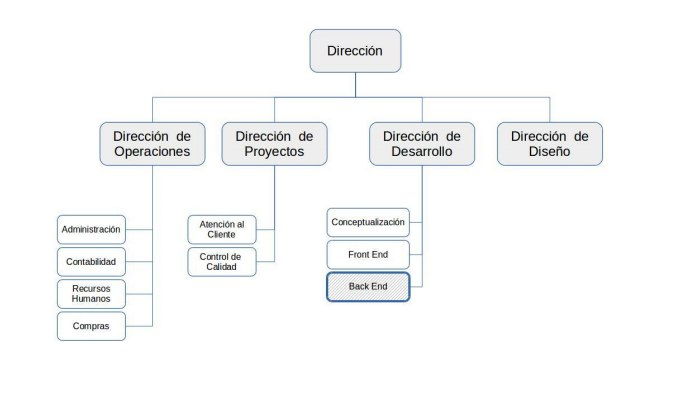
\includegraphics{Estructura_Turpial.png} \\


\subsection*{Ubicación del pasante}

El desarrollo de la pasantía fue llevado a cabo en la Dirección de Desarrollo de la empresa. El pasante fue asignado al departamento de \textit{Backend} bajo el cargo de Pasante, para cumplir tareas tales como: levantar requerimientos, diseñar y desarrollar las funcionalidades de la solución propuesta para el sistema. 



